%===========================================================================


\section{Label-Anchor Attribution \texorpdfstring{[E]}{[E]}}
\label{sec:label_anchor_results}
%===========================================================================

Variants A, B and C vary the label within Sepsis-3 and share the
culture-plus-antibiotic anchor, so H1 cannot distinguish an effect of reading
the definition differently (definitional) from an effect of choosing a
different construct (empirical). This section separates the two by labelling
each limb of the Sepsis-3 conjunction separately (Section~\ref{sec:alt_labels};
post-hoc, Protocol Amendment 2, exploratory family E3).

\subsection{The Anchor Determines Every Onset Time}

Under Variants A, B and C the onset time is the suspicion time
$t_{\text{susp}}$; the SOFA criterion determines only \emph{whether} a stay is
labelled, not \emph{when}. Variant E, which removes the SOFA criterion, is
therefore a strict superset of Variant B: every one of B's
\pcNPositiveBPanel{} labelled stays is also labelled by E, and in
\textbf{\pcPctExactMatchE\% of them the onset hour is identical}. Adding the
organ-dysfunction requirement discards \pcNPositiveEExcessOverB{} of E's
\pcNPositiveE{} labelled stays, two thirds, and moves not one onset
by a single hour.

\begin{table}[H]
    \centering\small
    \adjustbox{max width=\textwidth}{%
    \begin{tabular}{llrrrrr}
        \toprule
        \textbf{Var} & \textbf{Label} & \textbf{Onsets ($\leq$72\,h)} & \textbf{\%}
        & \textbf{$\kappa$ vs B} & \textbf{Sens.\ to B}
        & \textbf{Exact onset match} \\
        \midrule
        A & Narrow          & \pcNPositiveA  & \pcPctOnsetsAPanel  & \pcKappaVsBA & \pcSensToBA & \pcPctExactMatchA\% \\
        B & Seymour-Std     & \pcNPositiveBPanel & \pcPctOnsetsBPanel & n/a   & n/a   & n/a    \\
        C & Liberal         & \pcNPositiveC  & \pcPctOnsetsCPanel  & \pcKappaVsBC & \pcSensToBC & \pcPctExactMatchC\% \\
        \midrule
        E & Anchor-Only     & \pcNPositiveE  & \pcPctOnsetsEPanel  & \pcKappaVsBE & \textbf{\pcSensToBE} & \textbf{\pcPctExactMatchE\%} \\
        D & Deterioration   & \pcNPositiveD  & \pcPctOnsetsDPanel  & \textbf{\pcKappaVsBD} & \pcSensToBD & \textbf{\pcPctExactMatchD\%} \\
        F & Sepsis-3 Early  & \pcNPositiveF  & \pcPctOnsetsFPanel  & \pcKappaVsBF & \textbf{\pcSensToBF} & \pcPctExactMatchF\% \\
        \bottomrule
    \end{tabular}}
    \caption{Onset agreement with Variant B across all five comparison variants,
    on the \pcNStays{} shared stays. Counts are restricted to onsets inside the
    72\,h modelling horizon so that Variant D, whose onsets exist only within the
    panel, is comparable. ``Sens.\ to B'' is the fraction of B's labelled stays
    that the variant also labels; ``exact onset match'' is computed among stays
    labelled by both.}
    \label{tab:label_agreement}
\end{table}

Within Sepsis-3 (Table~\ref{tab:label_agreement}, top block), variants that
agree a stay is septic almost always agree on the hour: \pcPctExactMatchA\% for A, \pcPctExactMatchC\%
for C. The pre-registered label variance therefore concerns \emph{which
patients} rather than \emph{when}, since timing is fixed by the treatment anchor
in all three. That disagreement is substantial: A and B share only \pcSensToBA{} of B's septic stays
($\kappa = \pcKappaVsBA$) despite near-identical prevalence.

A label built from physiology alone (Variant D) agrees with Sepsis-3 at $\kappa = \pcKappaVsBD$, barely distinguishable from
chance, and matches B's exact onset hour in only \pcPctExactMatchD\% of the
stays both label, with a median absolute shift of \pcMedianAbsShiftHD\,hours
(IQR \pcIqrShiftLoHD{} to $+\pcIqrShiftHiHD$). The anchor-independent label
thus identifies largely different patients at different times.

Variant F keeps the construct and the patients but changes the onset timing.
It labels every stay B labels ($\kappa = \pcKappaVsBF$, the
shortfall being the \pcFNExtraInHorizon{} stays discussed above whose onset only
enters the horizon under the earlier rule) yet agrees with B on the exact hour
in just \pcPctExactMatchF\% of them: two defensible readings of the same
definition place about a quarter of Sepsis-3 onsets at a different hour on the
same patients.

\subsection{Discrimination Under Each Limb}

\begin{table}[H]
    \centering\small
    \begin{tabular}{lrrrr@{\hskip 1.5em}rrrr}
        \toprule
        & \multicolumn{4}{c}{\textbf{AUROC}} & \multicolumn{4}{c}{\textbf{AUPRC}} \\
        \cmidrule(lr){2-5}\cmidrule(lr){6-9}
        \textbf{Model} & \textbf{B} & \textbf{E} & \textbf{D} & \textbf{F}
                       & \textbf{B} & \textbf{E} & \textbf{D} & \textbf{F} \\
        \midrule
        Primary & \pcAurocPrimaryB & \pcAltAurocFullPrimaryE & \pcAltAurocFullPrimaryD & \pcAltAurocFullPrimaryF
                & \pcAuprcPrimaryB & \pcAltAuprcFullPrimaryE & \pcAltAuprcFullPrimaryD & \pcAltAuprcFullPrimaryF \\
        GBT     & \pcAurocGbtB     & \pcAltAurocFullGbtE     & \pcAltAurocFullGbtD     & \pcAltAurocFullGbtF
                & \pcAuprcGbtB     & \pcAltAuprcFullGbtE     & \pcAltAuprcFullGbtD     & \pcAltAuprcFullGbtF \\
        NEWS2   & \pcAurocNewsB    & \pcAltAurocFullNewsE    & \pcAltAurocFullNewsD    & \pcAltAurocFullNewsF
                & \pcAuprcNewsB    & \pcAltAuprcFullNewsE    & \pcAltAuprcFullNewsD    & \pcAltAuprcFullNewsF \\
        Cox     & \pcAurocCoxB     & \pcAltAurocFullCoxE     & \pcAltAurocFullCoxD     & \pcAltAurocFullCoxF
                & \pcAuprcCoxB     & \pcAltAuprcFullCoxE     & \pcAltAuprcFullCoxD     & \pcAltAuprcFullCoxF \\
        qSOFA   & \pcAurocQsofaB   & \pcAltAurocFullQsofaE   & \pcAltAurocFullQsofaD   & \pcAltAurocFullQsofaF
                & \pcAuprcQsofaB   & \pcAltAuprcFullQsofaE   & \pcAltAuprcFullQsofaD   & \pcAltAuprcFullQsofaF \\
        SIRS    & \pcAurocSirsB    & \pcAltAurocFullSirsE    & \pcAltAurocFullSirsD    & \pcAltAurocFullSirsF
                & \pcAuprcSirsB    & \pcAltAuprcFullSirsE    & \pcAltAuprcFullSirsD    & \pcAltAuprcFullSirsF \\
        \midrule
        \textbf{Events} & \pcNTestEventsB & \pcAltNEventsE & \pcAltNEventsD & \pcAltNEventsF & & & & \\
        \bottomrule
    \end{tabular}
    \caption{Discrimination under each limb of the Sepsis-3 conjunction and
    under standard onset timing (temporal test set, unrestricted window).
    B = Sepsis-3 (anchor \textbf{and} organ dysfunction); E = suspicion anchor
    only; D = organ dysfunction only, anchor-independent; F = Sepsis-3 with
    onset at $\min(t_{\text{susp}}, t_{\text{SOFA}})$. AUPRC is reported
    alongside AUROC because the four labels have very different prevalences.}
    \label{tab:label_anchor}
\end{table}

\begin{figure}[H]
    \centering
    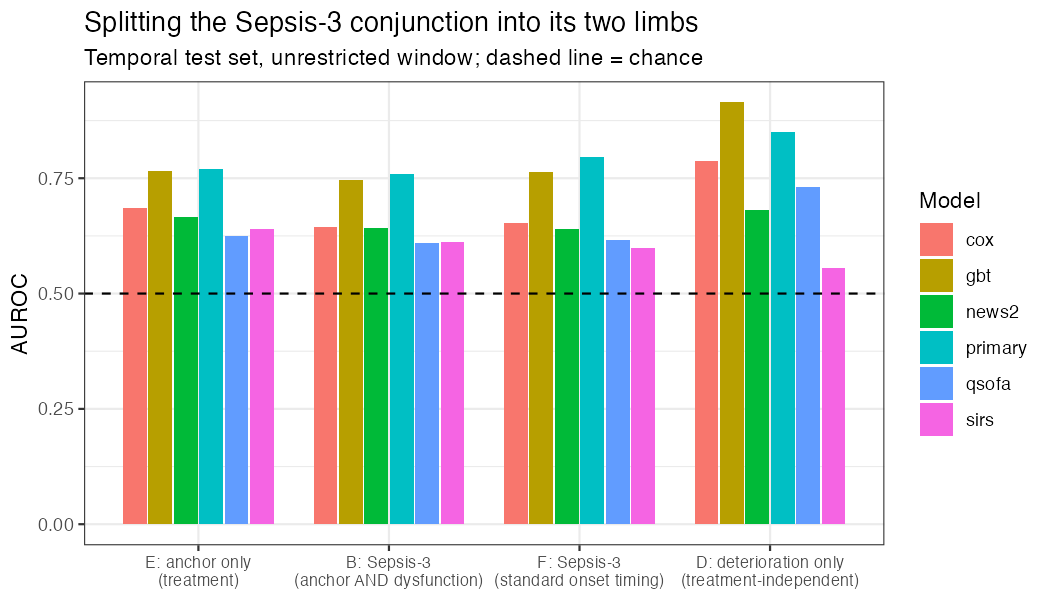
\includegraphics[width=0.9\textwidth]{images/09_label_anchor_attribution.png}
    \caption{Splitting the Sepsis-3 conjunction. The two limbs and the intact
    conjunction sit close together; only the anchor-independent deterioration
    label separates from them, and its level is not comparable with the others
    (Section~\ref{sec:variant_d_establishes}). The dashed line is chance.}
    \label{fig:label_anchor}
\end{figure}

\paragraph{Anchor-attributable fraction.}
The share of Sepsis-3's above-chance discrimination that the treatment anchor
reproduces on its own (Equation~\ref{eq:anchor_fraction}), with the ratio
bootstrapped end to end, is
\[
    \phi_{\text{anchor}} = \pcPhiAnchorPrimary
    \;\;[\pcPhiAnchorCiLoPrimary,\, \pcPhiAnchorCiHiPrimary]
    \quad\text{(primary)},\qquad
    \pcPhiAnchorGbt
    \;\;[\pcPhiAnchorCiLoGbt,\, \pcPhiAnchorCiHiGbt]
    \quad\text{(GBT)}.
\]
For the primary model the interval \textbf{includes 1}, and the underlying
contrast is not significant: E against B is
$\Delta = \pcAltDeltaPrimaryE$ [\pcAltDeltaCiLoPrimaryE,
\pcAltDeltaCiHiPrimaryE], $p_{\text{BH}} = \pcAltDeltaPBhPrimaryE$ in family E3.
For GBT the interval sits just above 1 ($\Delta = \pcAltDeltaGbtE$,
$p_{\text{BH}} = \pcAltDeltaPBhGbtE$), a small but detectable effect.

On this cohort the treatment anchor alone is therefore about as predictable as
Sepsis-3 itself. Dropping the organ-dysfunction requirement nearly triples the
event count (\pcAltNEventsE{} against \pcNTestEventsB) and leaves
discrimination essentially unchanged: the SOFA gate selects which stays are
labelled without selecting the more separable ones.

\paragraph{Anchor-independent label.}
Variant D differs substantially: $\Delta = \pcAltDeltaPrimaryD$
[\pcAltDeltaCiLoPrimaryD, \pcAltDeltaCiHiPrimaryD] for the primary model and
$\pcAltDeltaGbtD$ for GBT, both significant in family E3. Its AUPRC gap is
larger still (\pcAltAuprcFullPrimaryD{} against \pcAuprcPrimaryB), which matters
more at this prevalence. Because five of D's six SOFA components are model
inputs, part of this separation is self-fulfilling
(Section~\ref{sec:alt_labels}).

\paragraph{Onset timing.}
Variant F, whose label is Sepsis-3 unmodified in membership, is also
significantly more separable than B ($\Delta = \pcAltDeltaPrimaryF$
[\pcAltDeltaCiLoPrimaryF, \pcAltDeltaCiHiPrimaryF],
$p_{\text{BH}} = \pcAltDeltaPBhPrimaryF$). Its AUPRC is \emph{higher} than B's
despite a comparable event count, so this is not a prevalence artefact. Onsets
placed when organ dysfunction is first detectable are more separable from
surrounding at-risk hours than the same onsets placed at the clinician's
action. This is consistent with, but does not demonstrate, the physiological
signal preceding the clinical response, since predictors are binned to the
onset hour (Section~\ref{sec:limitations}).

\paragraph{Summary.}
Variant E produces discrimination similar to Variant B, and Variant F,
Sepsis-3 under standard onset timing, produces higher discrimination for the
primary model. Variant D produces substantially higher discrimination, but its
AUROC is not directly comparable, because the label is derived from variables
that overlap with the model inputs. Within Sepsis-3, reduced discrimination is
therefore associated more with an onset placed at the clinician's action than
with the conjunction itself.

\subsection{The Empty Pre-Treatment Window Is a Property of the Onset Rule}
\label{sec:pretreatment_label}

Under the onset rule of Variants A--C the pre-treatment window is empty by
construction (Section~\ref{sec:h3}). Table~\ref{tab:pretreatment_label}
reports its contents under alternative rules.

\begin{table}[H]
    \centering\small
    \adjustbox{max width=\textwidth}{%
    \begin{tabular}{llrrl}
        \toprule
        \textbf{Var} & \textbf{Label} & \textbf{Pre-treatment person-h}
        & \textbf{Onsets} & \textbf{AUROC (primary / GBT)} \\
        \midrule
        B & Seymour-Std   & \pcPreTreatPersonHoursVarB & \textbf{\pcPreTreatOnsetsVarB} & undefined \\
        E & Anchor-Only   & \pcPreTreatPersonHoursVarE & \textbf{\pcPreTreatOnsetsVarE} & undefined \\
        F & Sepsis-3 Early-Onset & \pcPreTreatPersonHoursVarF & \textbf{\pcPreTreatOnsetsVarF}
          & \pcPreTreatAurocPrimaryF{} / \pcPreTreatAurocGbtF \\
        D & Deterioration & \pcPreTreatPersonHoursVarD & \textbf{\pcPreTreatOnsetsVarD}
          & \pcPreTreatAurocPrimaryD{} / \pcPreTreatAurocGbtD \\
        \bottomrule
    \end{tabular}}
    \caption{Events in the treatment-anchored (pre-treatment) evaluation window.
    E's and B's zeros are entailed by Proposition~\ref{prop:h3}. Variant F holds
    the Sepsis-3 conjunction and the labelled stays fixed and changes only the
    onset timestamp to the standard $\min(t_{\text{susp}}, t_{\text{SOFA}})$;
    Variant D removes the infection anchor altogether.}
    \label{tab:pretreatment_label}
\end{table}

The zeros for E and B carry no information: E's onset is the anchor, and B is a
subset of E with identical onset times.

\paragraph{Variant F.}
Variant F shares Variant B's windows, SOFA threshold, evaluation window and all
\pcFNOnsets{} septic stays; only the timestamp differs. With that change, \pcFNMovedEarlier{}
onsets move earlier (\pcFPctMovedEarlier\%; median \pcFMedianShiftH\,h, largest
\pcFMaxShiftH\,h), \pcFNBeforeAnchor{} land before the first antibiotic or
culture across the cohort, and \pcPreTreatOnsetsVarF{} of those fall in the
temporal test set. Sepsis-3 onsets therefore do precede clinical action under
the standard timing, and the primary model identifies those hours at
\pcPreTreatAurocPrimaryF{} AUROC on the onset-hour estimand; whether they are
predictable \emph{in advance} cannot be assessed, because predictors are binned
to the onset hour (Limitation~\ref{lim:current_hour}). Because F's membership
is unmodified Sepsis-3, this result does not depend on the Variant D caveat.

\paragraph{Event count.}
Agreement between F and B is \pcPctAgreeBF\% ($\kappa = \pcKappaVsBF$), and the
discrepancy is one-directional. Within the
72-hour prediction horizon F labels \pcNPositiveF{} stays against B's
\pcNPositiveB, and every one of B's is among them: $F \supseteq B$. The
\pcFNExtraInHorizon{} additional stays are those whose $t_{\text{susp}}$ falls
after hour 72, so no model here ever sees a labelled event for them, but
whose SOFA rise occurred inside the window. The onset rule therefore determines
how many events a real-time model can be trained and tested on, as well as when
they are recorded.

\paragraph{Variant D.}
Variant D records \pcPreTreatOnsetsVarD{} pre-treatment onsets, more than F, as
expected of a label without the infection requirement, identified at
\pcPreTreatAurocPrimaryD{} AUROC (\pcPreTreatAurocGbtD{} for GBT). The caveat of
Section~\ref{sec:alt_labels} applies to that level but not to the event count.

\subsection{Exploratory Family E3: Intervals and Correction}

\begin{table}[H]
    \centering\small
    \begin{tabular}{llrlrl}
        \toprule
        \textbf{Var} & \textbf{Model} & \textbf{AUROC} & \textbf{95\% CI}
        & \textbf{$\Delta$ vs B} & \textbf{95\% CI ($\Delta$), $q_{\text{BH}}$} \\
        \midrule
        E & Primary & \pcAltAurocPrimaryE & \pcAltAurocCiPrimaryE & \pcAltDeltaPrimaryE & [\pcAltDeltaCiLoPrimaryE, \pcAltDeltaCiHiPrimaryE], $q = \pcAltDeltaPBhPrimaryE$ \\
        E & GBT     & \pcAltAurocGbtE & \pcAltAurocCiGbtE & \pcAltDeltaGbtE & [\pcAltDeltaCiLoGbtE, \pcAltDeltaCiHiGbtE], $q = \pcAltDeltaPBhGbtE$ \\
        D & Primary & \pcAltAurocPrimaryD & \pcAltAurocCiPrimaryD & \pcAltDeltaPrimaryD & [\pcAltDeltaCiLoPrimaryD, \pcAltDeltaCiHiPrimaryD], $q = \pcAltDeltaPBhPrimaryD$ \\
        D & GBT     & \pcAltAurocGbtD & \pcAltAurocCiGbtD & \pcAltDeltaGbtD & [\pcAltDeltaCiLoGbtD, \pcAltDeltaCiHiGbtD], $q = \pcAltDeltaPBhGbtD$ \\
        F & Primary & \pcAltAurocPrimaryF & \pcAltAurocCiPrimaryF & \pcAltDeltaPrimaryF & [\pcAltDeltaCiLoPrimaryF, \pcAltDeltaCiHiPrimaryF], $q = \pcAltDeltaPBhPrimaryF$ \\
        F & GBT     & \pcAltAurocGbtF & \pcAltAurocCiGbtF & \pcAltDeltaGbtF & [\pcAltDeltaCiLoGbtF, \pcAltDeltaCiHiGbtF], $q = \pcAltDeltaPBhGbtF$ \\
        \midrule
        B & Primary & \pcAurocPrimaryB & [\pcAurocCiLoPrimaryB, \pcAurocCiHiPrimaryB] & n/a & n/a \\
        B & GBT     & \pcAurocGbtB     & [\pcAurocCiLoGbtB, \pcAurocCiHiGbtB]         & n/a & n/a \\
        \bottomrule
    \end{tabular}
    \caption{Exploratory family E3: AUROC under each limb of the Sepsis-3
    conjunction with 95\% stay-level cluster-bootstrap intervals, and the
    paired difference against Variant B corrected by Benjamini--Hochberg across
    the family of $m = \pcAltFamilySize$ contrasts. All variants are labelled on the same test
    stays, so each difference is evaluated within replicate.}
    \label{tab:e3_contrasts}
\end{table}

Every contrast is positive, and two of the six do not survive correction. The
first, E against B for the primary model ($q = \pcAltDeltaPBhPrimaryE$), is the
basis of the anchor-attribution result above; the corresponding GBT contrast is
significant but small. The second is F against B for GBT ($\Delta =
\pcAltDeltaGbtF$, 95\% CI \pcAltDeltaCiLoGbtF--\pcAltDeltaCiHiGbtF,
$q = \pcAltDeltaPBhGbtF$): re-timing the onset separates the labels for the
primary model but not for the boosted one, so the gain in separability from
re-timing is model-specific. The pre-treatment event counts of
Section~\ref{sec:pretreatment_label} do not depend on this contrast.

These intervals quantify sampling uncertainty only. Prevalence differs by a
factor of \pcAltEventRatioPrimaryE{} (E) and \pcAltEventRatioPrimaryD{} (D)
relative to B, and Variant D's label overlaps the model's inputs, so the
intervals establish which orderings are stable, not that the labels measure
comparable constructs.
